%
% analysis, example programs
%

\chapter{Results}
\label{ch:results}
% \epigraph{Dionysus [is] the Master of Illusions, who could make a vine grow
% out grow out of a ship's plank, and in general enable his votaries to see the
% world as the world's not.}%
% {\textsc{---e.\ r.\ dodds}\\\textit{The Greeks and the Irrational}}

% \epigraph{If the immutable appears recast, then you yourself have been
% transformed.}%
% {\textsc{---r.\ scott bakker}\\\textit{The Judging Eye}}

\epigraph{Logic merely enables one to be wrong with authority}%
{\textsc{---the doctor}} %\\\textit{The Wheel in Space}}

% \begin{itemize}
%     \item performance \& analysis
%     \begin{itemize}
%       \item What is an optimisation? Describe the metrics considered.
%         \begin{itemize}
%           \item wall-clock time, parallel speedup??
%           \item instruction count
%           \item memory traffic (load/store/coalescing)
%           \item memory size (heap, register count, shared memory)
%           \item program size (number of parallel steps)
%           \item code size (generated binary, compilation time c.f. code complexity)
%         \end{itemize}
%     \end{itemize}
%
%     \item expressiveness / example programs
%     \item difficulties
%     \begin{itemize}
%         \item code generation
%         \item unintentional nesting
%     \end{itemize}
% \end{itemize}

The previous chapters discussed the design, implementation and optimisation of
the Accelerate language and CUDA backend. This chapter analyses the performance
of the implementation. Benchmarks were conducted on a single Tesla T10 processor
(compute capability 1.3, 30 multiprocessors = 240 cores at 1.3GHz, 4GB RAM)
backed by two quad core Xeon E5405 CPUs (64-bit, 2GHz, 8GB RAM) running
GNU/Linux (Ubuntu 12.04 LTS, CUDA 5.0).


\section{Runtime Overheads}

Runtime program optimisation, code generation, kernel loading, data transfer,
and so on can contribute significant overhead to short lived GPU computations.
Accelerate mitigates these overheads via caching and memoisation. For example,
the first time a particular expression is executed it is compiled to CUDA code,
which is reused for subsequent invocations. This section analyses those
overheads, so that they can be factored out later when we discuss the effects of
the program optimisations on kernel runtimes of the benchmark programs.


\subsection{Program Optimisation}

% tk: performance and benchmarks for the fusion pass
%   - actual runtime
%   - tick counters for the final version and old one with extend/cunctation
%     separation

\subsection{Data Transfer}

% tk: some graphs of memory transfer times or bandwith vs. array size
% tk: importance of using weak pointers, so data transfers ``escape'' the black
%     box of evaluating the AST --> hashcat.
% tk: importance of the nursery for reducing calls to malloc/free

\subsection{Code Generation \& Compilation}

% tk: measure \& tabulate some code generation / compilation times
% tk: persistent cache, perhaps just a mention?


\section{Dot product}

Dot product, or scalar product, is an algebraic operation that takes two
equal-length sequences of numbers and returns a single number by computing the
sum of the products of the corresponding entries in the two sequences. Dot
product can be defined in Accelerate using the code below, which was also seen
in section~\ref{sec:producer_consumer_fusion}.
%
\begin{lstlisting}[style=haskell
    ,label=lst:dotp
    ,caption={Vector dot-product in Accelerate}]
dotp :: Acc (Vector Float) -> Acc (Vector Float) -> Acc (Scalar Float)
dotp xs ys = A.fold (+) 0                       -- sum result of\ldots
           $ A.zipWith (*) xs ys                -- \ldots element-wise multiplying inputs
\end{lstlisting}
%
Figure~\ref{fig:dotp} show the result of running this code, compared to several
other sequential and parallel implementations. The \texttt{Data.Vector} baseline
is sequential code produced by \index{fusion!stream}stream
fusion~\cite{Coutts:2007kp}, running on the host CPU. The \texttt{Repa} version
runs in parallel on all eight cores of the host CPU, using the fusion method of
\index{fusion!delayed arrays}delayed arrays~\cite{Keller:2010er}. The
\texttt{NDP2GPU}~\cite{Bergstrom:2012bi} version compiles NESL
code~\cite{Blelloch:1995ut} down to CUDA. The performance of this version
suffers because the \texttt{NDP2GPU} compiler uses the legacy NESL compiler for
the front-end, which introduces redundant administrative operations that are not
strictly needed when evaluating a dot product.

\begin{figure}[htbp]
    \begin{center}
        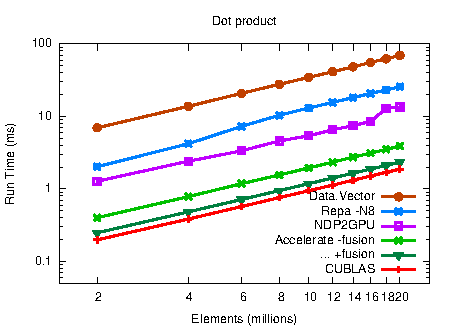
\includegraphics[width=0.8\textwidth]{images/sec-6/dotp/dotp}
    \end{center}
    \caption[Vector dot product kernel benchmarks]{Kernel runtimes for vector
        dot product, in Accelerate with and without optimisations, compared to
        other parallel GPU and CPU implementations. Note the log-log scale.}
    \label{fig:dotp}
\end{figure}

Without optimisations the Accelerate version executes in approximately twice the
time of the CUBLAS version. Since the individual aggregate operations consist of
only a single arithmetic operation each, the problem can not be a lack of
sharing.


\subsection{Too many kernels}

The slow-down in the unoptimised version is due to Accelerate generating one GPU
kernel function for each aggregate operation in the source program. The use of
two separate kernels requires the intermediate array produced by \code{zipWith}
to be constructed in GPU memory before being immediately read back by
\code{fold}. In contrast the CUBLAS version uses only a single kernel. As this
is a simple memory bound benchmark, lack of fusion roughly doubles the runtime.

The fused version of dot product combines the aggregate computations by
embedding a function of type \code{(sh -> a)} into the reduction, represented
here as the second argument to the constructor \code{Delayed}. This scalar
function does the work of element wise multiplying the two input vectors, and is
performed on-the-fly as part of the reduction kernel instead of requiring an
intermediate array:
%
\begin{lstlisting}[style=haskell]
let a0 = use (Array ...) in
let a1 = use (Array ...) in
fold (\x0 x1 -> x0 + x1) 0.0
   (Delayed (intersect (shape a0) (shape a1))   -- extent of the input array
            (\x0 -> (a0!x0) * (a1!x0)))         -- function to generate a value at each index
\end{lstlisting}

While the fused Accelerate version is $30\times$ faster than the sequential
version executed on the CPU, it is still approximately $20\%$ slower than the
hand-written CUBLAS version. As dot product is a computationally simple task,
any additional overheads in the implementation will be significant. To see why
this version is still slightly slower, we analyse the generated code to inspect
it for sources of overhead.


\subsection{Duplicate loop counters}

The fused dot product operation will only perform the element wise
multiplication of the two input arrays in the first step of the tree reduction
(\S\ref{sec:parallel_reduction}). This occurs in the phase of the cascaded
algorithm when individual threads sequentially sum multiple elements. After
embedding the fused producer, the following CUDA code is generated for the inner
loop of this step:
%
% pookie is the bestest
% bubbaboo ish silly
% kekekee
% i can't put smiley faces in cause weird things happen
% hehe^{this is my thesis
% please like it
% i worked really hard
% and writed a lots
% }<++>
%
%
\begin{lstlisting}[style=cuda
    ,firstnumber=18
    ,label=lst:dotp_cuda
    ,caption={Generated CUDA code for the first step of fused dot product}]
for (ix += gridSize; ix < shapeSize; ix += gridSize) {
    const Int64 v2 = ix;
    const int v3 = toIndex(shIn0, shape(v2));
    const int v4 = toIndex(shIn1, shape(v2));

    x0 = arrIn0_a0[v3] * arrIn1_a0[v4];
    y0 = x0 + y0;
}
\end{lstlisting}
%
We have four loop counters: \code{ix}, \code{v2}, \code{v3} and \code{v4} ---
two for the source arrays and two to convert between the multidimensional and
linear representations. These counters contain the same value and are
incremented in lockstep. In addition to the superfluous arithmetic, the
duplication of counters unnecessarily increases register pressure.

\marginnote{this was unexpected}
The corresponding section of PTX~\cite{NVIDIA:2012vj} code is for this loop is
shown in Listing~\ref{lst:dotp_ptx}. To retrieve the data from the first input
array, the input array pointer is retrieved (line~\ref{lst:dotp_ptx_ldparam}),
the offset stored in register \code{rd16} added to it
(line~\ref{lst:dotp_ptx_add}), and then the value read from global memory at
this address (line~\ref{lst:dotp_ptx_ldglobal}). Happily, we note that
retrieving the second input element \emph{also} uses the offset stored in
register \code{rd16} (line~\ref{lst:dotp_ptx_ldglobal2}).
%
\begin{lstlisting}[style=ptx
    ,float
    ,firstnumber=103
    ,label=lst:dotp_ptx
    ,caption={[Corresponding PTX code for the first step of fused dot product]
        Corresponding PTX code for the first step of fused dot product (sm13)}]
 //  18          for (ix += gridSize; ix < shapeSize; ix += gridSize) {
        cvt.u32.u16     %r10, %nctaid.x;
        mul.lo.u32      %r11, %r10, %r1;
        add.s32         %r12, %r11, %r7;
        mov.s32         %r13, %r12;
        setp.le.s32     %p2, %r8, %r12;
        @%p2 bra        $Lt_0_13058;
        cvt.s64.s32     %rd12, %r12;
        cvt.s64.u32     %rd13, %r11;
$Lt_0_14082:
 //<loop> Loop body line 18, nesting depth: 1, estimated iterations: unknown
        .loc    16      24      0
 //  20              const int v3 = toIndex(shIn0, shape(v2));
 //  21              const int v4 = toIndex(shIn1, shape(v2));
 //  22
 //  23              x0 = arrIn0\_a0[v3] * arrIn1\_a0[v4];
 //  24              y0 = x0 + y0;
        cvt.s32.s64     %rd14, %rd12;                           (@* \label{lst:dotp_ptx_cvt1} *@)
        cvt.s32.s64     %r14, %rd14;
        cvt.s64.s32     %rd15, %r14;                            (@* \label{lst:dotp_ptx_cvt3} *@)
        mul.wide.s32    %rd16, %r14, 4;
        .loc    16      17      0
        ld.param.u64    %rd9, [__cudaparm_foldAll_arrIn0_a0];   (@* \label{lst:dotp_ptx_ldparam} *@)
        .loc    16      24      0
        add.u64         %rd17, %rd16, %rd9;                     (@* \label{lst:dotp_ptx_add} *@)
        ld.global.f32   %f4, [%rd17+0];                         (@* \label{lst:dotp_ptx_ldglobal} *@)
        .loc    16      17      0
        ld.param.u64    %rd8, [__cudaparm_foldAll_arrIn1_a0];
        .loc    16      24      0
        add.u64         %rd18, %rd16, %rd8;
        ld.global.f32   %f5, [%rd18+0];                         (@* \label{lst:dotp_ptx_ldglobal2} *@)
        mad.f32         %f3, %f4, %f5, %f3;
        add.s32         %r13, %r13, %r11;
        add.s64         %rd12, %rd12, %rd13;
        setp.gt.s32     %p3, %r8, %r13;
        @%p3 bra        $Lt_0_14082;
        bra.uni         $Lt_0_13058;
$Lt_0_13314:
        mov.f32         %f3, %f6;
$Lt_0_13058:
        .loc    16      27      0
 //  25          }
\end{lstlisting}

In this case the CUDA compiler was able to coalesce our four counters into a
single counter. This is because our definition of \code{toIndex} specialised for
one-dimensional indices \code{DIM1} does \emph{not} do bounds checking:
%
\begin{lstlisting}[style=cuda]
template <>
static __inline__ __device__ Ix toIndex(const DIM1 sh, const DIM1 ix)
{
    return ix;
}
\end{lstlisting}
%
Since we do not check that the current index \code{ix} is within bounds of the
array shape \code{sh}, the compiler can see that the definitions of \code{v3}
and \code{v4} in Listing~\ref{lst:dotp_cuda} are identical. Similarly
one-dimensional indices are just integers, and so the one-dimensional instance
of \code{shape} is the identity function. For higher dimensional shapes,
however, this is not the case and \code{toIndex} and \code{shape} do real work
to their arguments. As the shape \code{shIn0} and \code{shIn1} are inputs
arguments to the kernel, the compiler will not be able to determine they are
equivalent and so the counters would not be combined.

Why don't we perform bounds checks in \code{toIndex}? Implementing exceptions in
a massively parallel architecture is difficult, and support for throwing
exceptions from kernel functions was only recently added for devices of compute
capability 2.0 and later~\cite{NVIDIA:2012wf}. % [\SB.15]


\subsection{64-bit Arithmetic}

CUDA devices are at their core 32-bit processors and thus are optimised for
32-bit arithmetic. For example, our Tesla GPU with compute capability 1.3 has a
throughput of eight 32-bit floating-point add, multiply, or multiply-add
operations per clock cycle per multiprocessor, but only a single operation per
cycle of the 64-bit equivalents of these~\cite{NVIDIA:2012wf}. % [\S5.4.1]

However, the host architecture that the Haskell program executes on is likely to
be a 64-bit processor. This means that an \code{Int} value from Haskell ---
which may appear marshalled as array data or shape values --- will generate code
to manipulate 64-bit integers, as well as conversions between 32- and 64-bit
types. Lines~\ref{lst:dotp_ptx_cvt1}--\ref{lst:dotp_ptx_cvt3} of
Listing~\ref{lst:dotp_ptx} contain such type conversions, which on our compute
capability 1.3 device have a throughput of only a single operation per cycle per
multiprocessor. These conversions would not be necessary if we were not
cross-compiling from a 64-bit Haskell host, or if the programmer working
directly with CUDA only used the \code{int} type, which would be interpreted by
the CUDA compiler as a 32-bit wide integer.


\subsection{Non-neutral starting elements}

For convenience, and to avoid possibly unexpected behaviour, Accelerate's
\code{fold*} family of functions do not require the combination function and
starting element to form a moniod. We still require the function to be
associative, so that the reduction can be implemented efficiently in parallel as
a tree-reduction, but the initial element does not need to be a \emph{neutral}
element.\marginnote{semigroup?} For example, \code{fold (+) 10} is valid in
Accelerate and evaluates to the correct answer.

However, this means that evaluation of the reduction is more complex. In
particular, we can not simply initialise all threads to the initial value.
In the first phase of the reduction, threads must be sure to initialise
their local sum \code{y0} with values from the input array before beginning the
sequential loop show in Listing~\ref{lst:dotp_cuda}:
%
% tk: hacks in comment style below: check if changing the basic language style
\begin{lstlisting}[style=cuda,firstnumber=12]
if (ix < shapeSize) {
    const Int64 v2 = ix;
    const int v3 = toIndex(shIn0, shape(v2));
    const int v4 = toIndex(shIn1, shape(v2));

    y0 = arrIn0_a0[v3] * arrIn1_a0[v4];
    for (ix += gridSize; ix < shapeSize; ix += gridSize) {
\end{lstlisting}

Similarly, in the second parallel tree reduction phase threads may only read
values from shared memory that were properly initialised. This requires
additional bounds checks at every step:
%
\begin{lstlisting}[style=cuda,firstnumber=27]
sdata0[threadIdx.x] = y0;
__syncthreads();
ix = min(shapeSize - blockIdx.x * blockDim.x, blockDim.x);
if (threadIdx.x + 512 < ix) {
    x0 = sdata0[threadIdx.x + 512];
    y0 = y0 + x0;
    sdata0[threadIdx.x] = y0;
}
__syncthreads();
if (threadIdx.x + 256 < ix) {
    x0 = sdata0[threadIdx.x + 256];
    y0 = y0 + x0;
    sdata0[threadIdx.x] = y0;
}
__syncthreads();
// etc...
\end{lstlisting}

These requirements increase overhead from ancillary instructions that are not
loads, stores, or arithmetic for the core computation. A summation reduction has
low arithmetic intensity to begin with, and is the limiting factor in the
performance of this kernel, so additional bounds checks further reduce
performance.

\subsection{Kernel specialisation}

To further reduce instruction overhead, it is possible to completely unroll the
reduction by specialising the kernel for a specific block size. In standard CUDA
this can be achieved through the use of C++ templates. Branches referring to the
template parameter will be evaluated at compile time, resulting in a very
efficient inner loop.
%
\begin{lstlisting}[style=cuda]
template <unsigned int blockSize> __global__ void reduce(...) {
    ...
    if (blockSize > 512) {
    }
    if (blockSize > 256) {
    }
    ...
\end{lstlisting}

This technique has shown to produce significant gains in
practice~\cite{Harris:2007te}, although requires compiling a separate kernel for
each thread block size we wish to specialise for. Accelerate can achieve this
kind of kernel specialisation because the CUDA code is generated at program
runtime, but this extra compilation adds significant additional overhead. Since
compiled kernels are cached and reused (\S tk), if we know that the reduction
will be computed many times the extra compilation overhead can be amortised by
the improved kernel performance, and may thus be worthwhile. Such
specialisations are left for future work.


\section{Black-Scholes option pricing}

The Black-Scholes algorithm is a partial differential equation for modelling the
evolution of a European-style stock option price under certain assumptions. The
corresponding Accelerate program is shown in Listing~\ref{lst:blackscholes}.
Given a vector of triples of the underlying stock price, strike price, and time
to maturity in years, the Black-Scholes formula computes the price of a call and
put option. The function \code{callput} evaluates the Black-Scholes formula for
a single triple, and \code{blackscholes} maps it over a vector of triples such
that all individual applications of the formula are executed in parallel.
%
\begin{lstlisting}[style=haskell
    ,float=tbh
    ,label=lst:blackscholes
    ,caption={Black-Scholes option pricing in Accelerate}]
horner :: Num a => [a] -> a -> a
horner coeff x =
  let madd a b  = a + x*b
  in
  x * foldr1 madd coeff

cnd' :: Floating a => a -> a
cnd' d =
  let poly      = horner coeff
      coeff     = [0.31938153, -0.356563782, 1.781477937, -1.821255978, 1.330274429]
      rsqrt2pi  = 0.39894228040143267793994605993438
      k         = 1.0 / (1.0 + 0.2316419 * abs d)
  in
  rsqrt2pi * exp (-0.5*d*d) * poly k

blackscholes :: Acc (Vector (Float, Float, Float)) -> Acc (Vector (Float, Float))
blackscholes = A.map callput
  where
  callput x =
    let (price, strike, years) = A.unlift x
        r       = A.constant riskfree
        v       = A.constant volatility
        v_sqrtT = v * sqrt years
        d1      = (log (price / strike) + (r + 0.5 * v * v) * years) / v_sqrtT
        d2      = d1 - v_sqrtT
        cnd d   = let c = cnd' d in d >* 0 ? (1.0 - c, c)
        cndD1   = cnd d1
        cndD2   = cnd d2
        x_expRT = strike * exp (-r * years)
    in
    A.lift ( price * cndD1 - x_expRT * cndD2                    -- call price
           , x_expRT * (1.0 - cndD2) - price * (1.0 - cndD1))   -- put price
\end{lstlisting}

Figure~\ref{fig:blackscholes} shows the result of running this code compared to
the implementation that ships with the CUDA SDK. Without optimisations, the
Accelerate version is almost twenty times slower than the equivalent
implementation in CUDA C. As \code{blackscholes} includes only one collective
array operation, the problem can not be a lack of fusion.

\begin{figure}[htbp]
    \begin{center}
        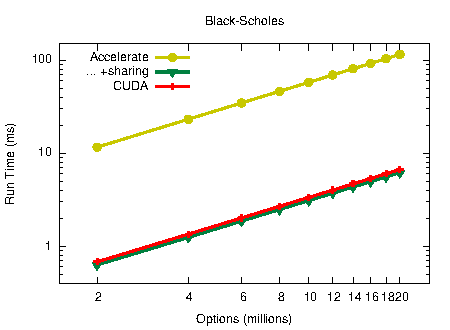
\includegraphics[width=0.8\textwidth]{images/sec-6/black-scholes/black-scholes}
    \end{center}
    \caption[Black-Scholes kernel benchmarks]{Kernel runtimes for Black-Scholes
        options pricing, in Accelerate with and without optimisations, compared
        to a hand-written CUDA version. Note the log-log scale.}
    \label{fig:blackscholes}
\end{figure}

\subsection{Too little sharing}

The function \code{callput} from Listing~\ref{lst:blackscholes} includes a
significant amount of sharing: the helper functions \code{cnd'} and hence
\code{horner} are used twice --- for \code{d1} and \code{d2} --- and its
argument \code{d} is used multiple times in the body. Furthermore, the
conditional expression \code{d >* 0 ? (1 - c, c)} results in a branch that,
without sharing, results in a growing number of predicated instructions that
leads to a large penalty on the SIMD architecture of the GPU.

Without sharing the generated code requires 2573 instructions and results in
\marginnote{check instruction count difference}
significant warp divergence which serialises portions of the execution. With
sharing recovery the generated code requires 501 instructions and is actually
slightly faster than the reference CUDA version because the latter contains a
common subexpression that is not spotted by the programmer and not eliminated by
the CUDA compiler. The common subexpression performs a single multiplication.


\section{Mandelbrot fractal}
\label{sec:mandelbrot}

The Mandelbrot set is generated by sampling values $c$ in the complex plane and
determining whether under iteration of the complex quadratic polynomial:
\[
z_{n+1} = z_{n}^{2} + c
\]
that the magnitude of $z$ (written $\left| z_{n} \right|$) remains bounded
however large $n$ gets. Images of the Mandelbrot set are created such that each
pixel corresponds to a point $c$ in the complex plane, and its colour depends on
the number of iterations $n$ before the relation diverges, with $z_{0} = c$. The
set of points forming the boundary of this relation forms the distinctive and
easily recognisable fractal shape, as was seen in Figure~\ref{fig:mandelbrot}.

\begin{table}
    \centering
    \small
    \begin{tabular}{lrrrr}

                        & \multicolumn{1}{c}{Time}
                        & \multicolumn{1}{c}{Bandwidth}
                        & \multicolumn{1}{c}{Step}
                        & \multicolumn{1}{c}{Cumulative} \\

\textbf{Benchmark}      & \multicolumn{1}{c}{(ms)}
                        & \multicolumn{1}{c}{(GB/s)}
                        & \multicolumn{1}{c}{Speedup}
                        & \multicolumn{1}{c}{Speedup} \\\hline

Accelerate              &
                        &
                        &
                        & \\

Accelerate (+sharing)   &
                        &
                        &
                        & \\

Accelerate (+fusion)    &
                        &
                        &
                        & \\

Accelerate (+loop recovery)
                        &
                        &
                        &
                        & \\

CUDA (limit)            & 14.0
                        & 0.55
                        &
                        & \\

CUDA (avg)              & 5.0
                        & 1.53
                        & 2.79$\times$
                        & 2.79$\times$ \\

CPU (avg)               & 1389
                        & 0.006
                        &
                        & \\

    \end{tabular}
    \caption[Mandelbrot fractal kernel benchmarks]{Mandelbrot fractal benchmarks
        in Accelerate with and without optimisations, compared to a hand written
        CUDA version. \note{tk: figure?}}
    \label{tab:mandelbrot}
\end{table}

As expected, Table~\ref{tab:mandelbrot} shows that without fusion performance is
poor because storing each step of the iteration saturates the memory bus to the
point that reducing arithmetic intensity with sharing recovery
(\S\ref{sec:sharing_observation}) provides no improvement.


\subsection{Fixed unrolling}

In order to meet the restrictions of what can be efficiently executed on
specialised hardware such as GPUs, Accelerate does not directly support any form
of recursion. To implement the recurrence relation we instead define each step
as a collective operation and unfold the loop a fixed number of times.

Given $z_{n}$ and $c$, we can easily compute $z_{n+1}$, and for each point we
need to iterate this process until divergence, and then remember the number of
iterations at which divergence happened. This creates a small problem: GPUs are
designed to do the \emph{same thing} to lots of different data at the same time,
whereas we want to do something different depending on whether or not a
particular point has diverged or not.

Conditionals in GPU code should be avoided as much as possible because they can
lead to SIMD divergence. We can't avoid \emph{some} kind of conditional, but we
can make sure there is only a bounded amount of divergence by having just one
conditional per iteration, and a fixed number of iterations. The trick is to
keep a pair \code{(z,i)} for every array element, where \code{i} is the
iteration at which the point \code{z} diverged. Each step of the iteration is
then:
%
\begin{itemize}
    \item Compute \code{z' = c `plus` (z `times` z)}
    \item If \code{z'} is greater than 4, then the result is \code{(z, i)}
    \item Otherwise the result is \code{(z', i+1)}
\end{itemize}

\begin{lstlisting}[style=haskell
    ,float=tbh
    ,label=lst:mandelbrot
    ,caption={Mandelbrot set generator in Accelerate}]
type Complex = (Float, Float)                   -- not all GPUs can use \emph{Double}

mandelbrot :: Int -> Int -> Int -> Int
           -> Acc (Scalar View)
           -> Acc (Array DIM2 (Complex, Int))
mandelbrot screenX screenY depth view
  = P.foldr ($) zs0                             -- apply in sequence the\ldots  \label{lst:mandelbrot_foldr}
  $ P.take depth (repeat step)                  -- \ldots\emph{depth} copies of the function \emph{step}
  where
    cs  = genPlane screenX screenY view         -- the static complex plane $c$
    zs0 = mkinit cs                             -- initial array of $(c, 0)$

    step :: Acc (Array DIM2 (Complex, Int))     % \label{lst:mandelbrot_step} %
         -> Acc (Array DIM2 (Complex, Int))
    step = A.zipWith iter cs                    -- compute one iteration to progress to $z_{n+1}$

iter :: Exp Complex -> Exp (Complex, Int) -> Exp (Complex, Int)
iter c zi = f (A.fst zi) (A.snd zi)
 where
  f :: Exp Complex -> Exp Int -> Exp (Complex, Int)
  f z i =
    let z' = next c z
    in (dot z' >* 4) ? ( zi , lift (z', i+1) )

next :: Exp Complex -> Exp Complex -> Exp Complex
next c z = c `plus` (z `times` z)

dot :: Exp Complex -> Exp Float
dot = lift1 f
  where f :: (Exp Float, Exp Float) -> Exp Float
        f (x,y) = x*x + y*y
\end{lstlisting}

The core of the Mandelbrot routine is shown in Listing~\ref{lst:mandelbrot}. The
function \code{step} (Line~\ref{lst:mandelbrot_step}) advances the entire
complex plane by one iteration of the recurrence relation. This function is
replicated \code{depth} times and then the sequence combined by folding with the
function application operator \code{(\$)} (Line~\ref{lst:mandelbrot_foldr}). This
results in a single fused kernel whole performance is greatly improved, but
still several times slower than the CUDA version.

The slowdown is because the fused code generates a completely unrolled loop,
with \code{depth = 255} copies of the code for \code{step}. Unrolling loops not
only increases instruction count but can often increase register lifetimes
because of the scheduling of loads and stores. In particular, stores are pushed
down and loads are moved up in the instruction stream, which results in
temporary scalar lifetimes being longer. The unrolled code requires 63 registers
per thread (compute capability 3.0), resulting in a multiprocessor occupancy of
only 50\%. Since the Mandelbrot program is limited by computation, halving the
maximum number of resident threads halves the maximum performance.

% \begin{lstlisting}[style=cuda
%     ,firstnumber=24]
% const float v13 = v10 * v10 - v11 * v11;                // single application of \texttt{step}
% const float v14 = v10 * v11 + v11 * v10;
% const float v15 = v8 + v13;
% const float v16 = v9 + v14;
% const Word8 v17 = v15 * v15 + v16 * v16 > 4.0f;
% const float v18 = v17 ? v10 : v15;
% const float v19 = v17 ? v11 : v16;
% const Int64 v20 = v17 ? v12 : (Int64) 1;
%   // repeats 255 times\ldots
% \end{lstlisting}


\subsection{Loop recovery}

Sometimes unrolling loops can be beneficial. A CUDA programmer can control how
aggressively the compiler unrolls loops using the \code{#pragma unroll}
directive with an explicit unroll factor, where zero means to not unroll the
loop at all.

The problem is that the way we have fused the collective operations does not
preserve the iteration structure of the recurrence relation, so the loop is
completely unrolled in the single fused operation. We can re-introduce scalar
loops by analysing the fused expression to look for the following pattern:
%
\begin{lstlisting}[style=Haskell,numbers=none,mathescape]
%\bf$\langle$ loop introduction $\rangle$%
    let x =
        let y = e1
        in e2
    in e3
    $\mapsto$
    iterate[2] (\y -> e2) e1            %\rm if \texttt{e2} $\equiv$ \texttt{e3}%
\end{lstlisting}
%
The nested bindings are replaced with an explicit scalar value iteration
structure, where the expression \code{e2} is repeated twice with the initial
value \code{e1}. Similarly, loops can be joined:
%
\begin{lstlisting}[style=Haskell,numbers=none,mathescape]
%\bf$\langle$ loop joining $\rangle$%
    let x = iterate[n] (\y -> e2) e1
    in e3
    $\mapsto$
    iterate[n+1] (\y -> e2) e1          %\rm if \texttt{e2} $\equiv$ \texttt{e3}%
\end{lstlisting}
%
Recovering scalar loops in this way enables a backend to generate explicit loops
in the target language, and the compiler makes the decision of whether or not to
unroll the loop. In future, it would be beneficial to augment it with related
loop optimisations such as loop invariant code motion in the frontend and
lower-level code generation optimisations in a backend.


\subsection{Unbalanced workload}

The final problem with the Mandelbrot program is due to the initial formulation
of the program using a fixed unrolling, as we must handle application of the
function to elements which have already diverged. As explained, this is to
ensure that all threads [in a warp] continue doing the same thing, which avoids
excessive SIMD divergence, but means that the computation always proceeds to the
iteration limit.

For the Mandelbrot program threads only diverge in the sense that they are
either still computing the recurrence relation, or the point is not in the set
and the computation has completed; threads do not diverge to follow separate
execution paths. The latter type of SIMD divergence is what we really need to
avoid, because this results in predicated execution: threads taking the
\code{true} path of a branch execute while all other threads sit idle, then
execution switches to the \code{false} branch while the first set of threads
idle.

The CUDA version is faster because threads exit the loop as soon as their point
in the complex plane diverges. Although once a thread completes it sits idle
until all threads in the group complete their calculation, if all the points
within a group of threads diverge quickly this can save a significant amount of
work. Table~\ref{tab:mandelbrot} shows the difference in execution time when
displaying the entire fractal (avg), where points diverge at varying iteration
depths in the sequence, compared to a region where all thread continue to the
iteration limit (limit). In order to manage this unbalanced workload, the CUDA
version additionally includes a custom thread block scheduler.

This test demonstrates that while loop recovery offered a significant
performance benefit for free, it would be beneficial to expose looping
constructs in the source language as well, rather than relying on potentially
fragile post-hoc transformations. Avoiding thread divergence in CUDA programs is
an active area of research~\cite{Zhang:2010jc}.

\section{N-body gravitational simulation}

\begin{figure}[htbp]
    \begin{center}
        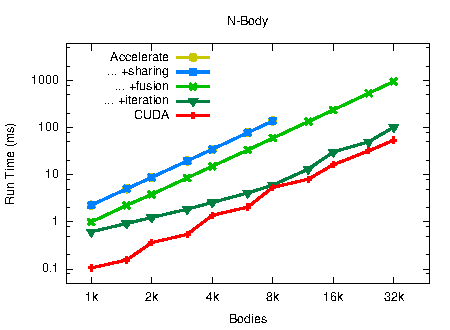
\includegraphics[width=0.8\textwidth]{images/sec-6/nbody/nbody}
    \end{center}
    \caption[N-body gravitational simulation kernel benchmarks]{Kernel runtimes
        for the $n$-body gravitational simulation, in Accelerate with and
        without optimisations, compared to a hand-written CUDA implementation.
        Note the log-log scale.}
    \label{fig:nbody}
\end{figure}

The $n$-body example simulates the Newtonian gravitational forces on a set of
massive bodies in 3D space, using the na\"ive $\mathcal{O}\left( n^{2} \right)$
algorithm. In a data-parallel setting, the natural way to express this algorithm
is first to compute the forces between every pair of bodies, before adding the
forces applied to each body using a segmented sum. Without fusion this approach
also requires $\mathcal{O}\left( n^{2} \right)$ space for the intermediate array
of forces, which exhausts the memory of our device (4GB!) when using more than
about five thousand bodies. With fusion, the reduction operation consumes each
force value on-the-fly, so that the program only needs $\mathcal{O}\left( n
\right)$ space to store the final force values. The core of the $n$-body
simulation is shown below, where \code{accel} calculates the acceleration
between two particles, and \code{(.+.)} component-wise sums the acceleration of
a particle along each $x$, $y$ and $z$ axis.

\begin{lstlisting}[style=haskell
    ,label=lst:nbody
    ,caption={$N$-body gravitational simulation in Accelerate}]
calcAccels :: Exp R -> Acc (Vector Body) -> Acc (Vector Accel)
calcAccels epsilon bodies
  = let n       = A.size bodies
        cols    = A.replicate (lift $ Z :. n :. All) bodies
        rows    = A.replicate (lift $ Z :. All :. n) bodies
    in
    A.fold (.+.) (vec 0) $ A.zipWith (accel epsilon) rows cols
\end{lstlisting}

\subsection{Use of Shared Memory}

Even with fusion the reference CUDA version is over 10x faster. In CUDA, the
memory hierarchy of the device is made explicit to the programmer, including a
small on-chip shared memory region threads can use to communicate results, that
is essentially a software managed cache (\S tk). The CUDA version uses this
memory region to share the particle mass and position data between a group of
threads, whereas Accelerate uses this region to share computation.

The CUDA version uses this low-latency memory region to reduce the bandwidth
requirements of the program by sharing the particle mass and position data
between the group of threads. This reduces the bandwidth requirement of the
program by a factor of the number of threads in a block (256) but requires each
thread to sum its particle interactions sequentially in $\mathcal{O}\left( n
\right)$ time. The Accelerate version uses shared memory to perform a
tree-reduction in $\mathcal{O}\left( \log n \right)$ time
(\S\ref{sec:parallel_reduction}) but requires all $n^{2}$ memory transfers. For
this bandwidth bound application, making the trade-off of parallelism for
bandwidth clearly wins. Automatic use of shared memory is a separate
consideration to the optimisations discussed in this work, and remains an open
research problem~\cite{Ma:2010ft}.


\section{Fluid Flow}

The fluid flow example implements Jos Stam's stable fluid
algorithm~\cite{Stam:1999ey}, which is a fast approximate algorithm intended for
animation and games, rather than accurate engineering simulation. An example
sequence is shown in Figure~\ref{fig:fluid_steps}.

\begin{figure}[htbp]
    \begin{center}
        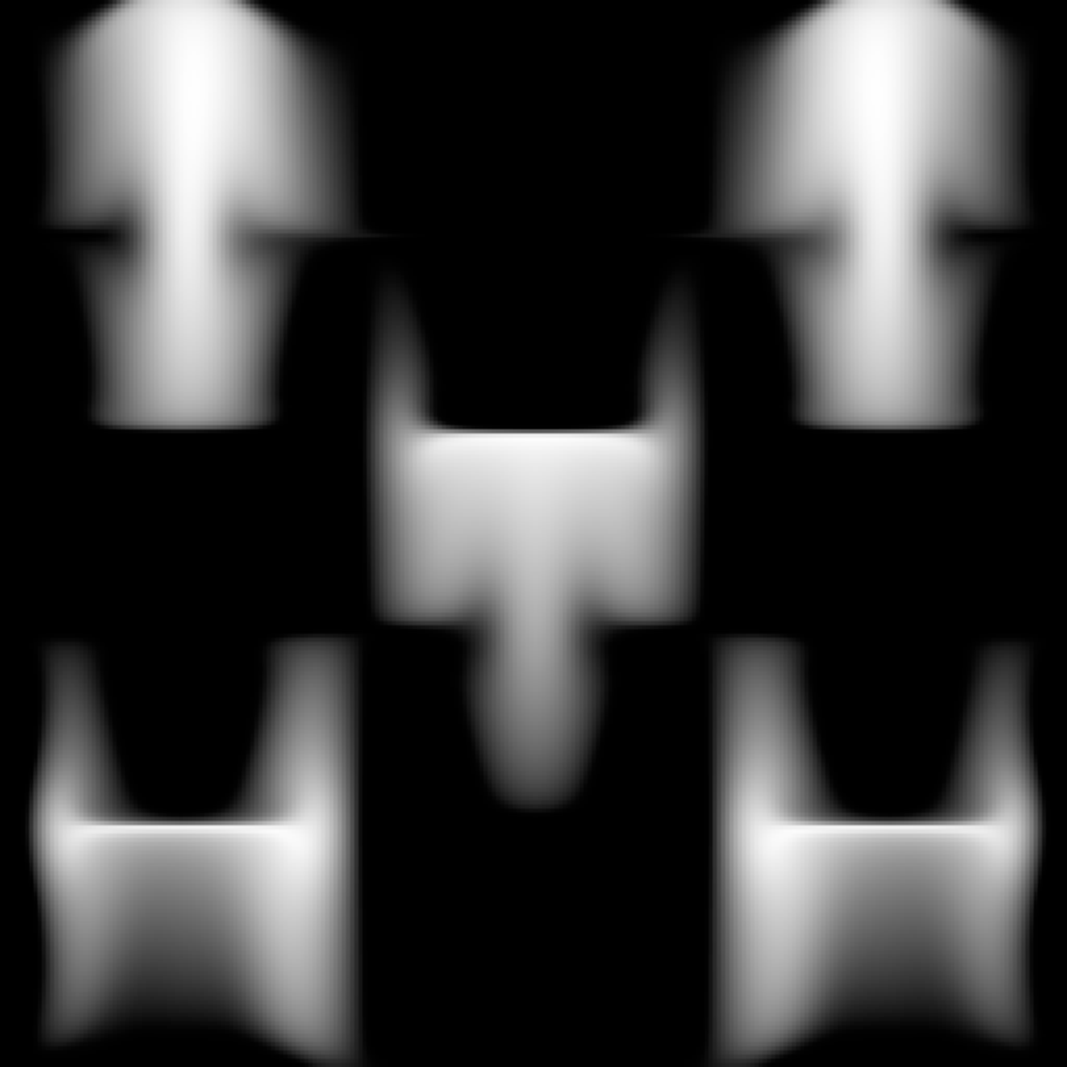
\includegraphics[width=0.3\textwidth]{images/sec-6/fluid/fluid-10}
        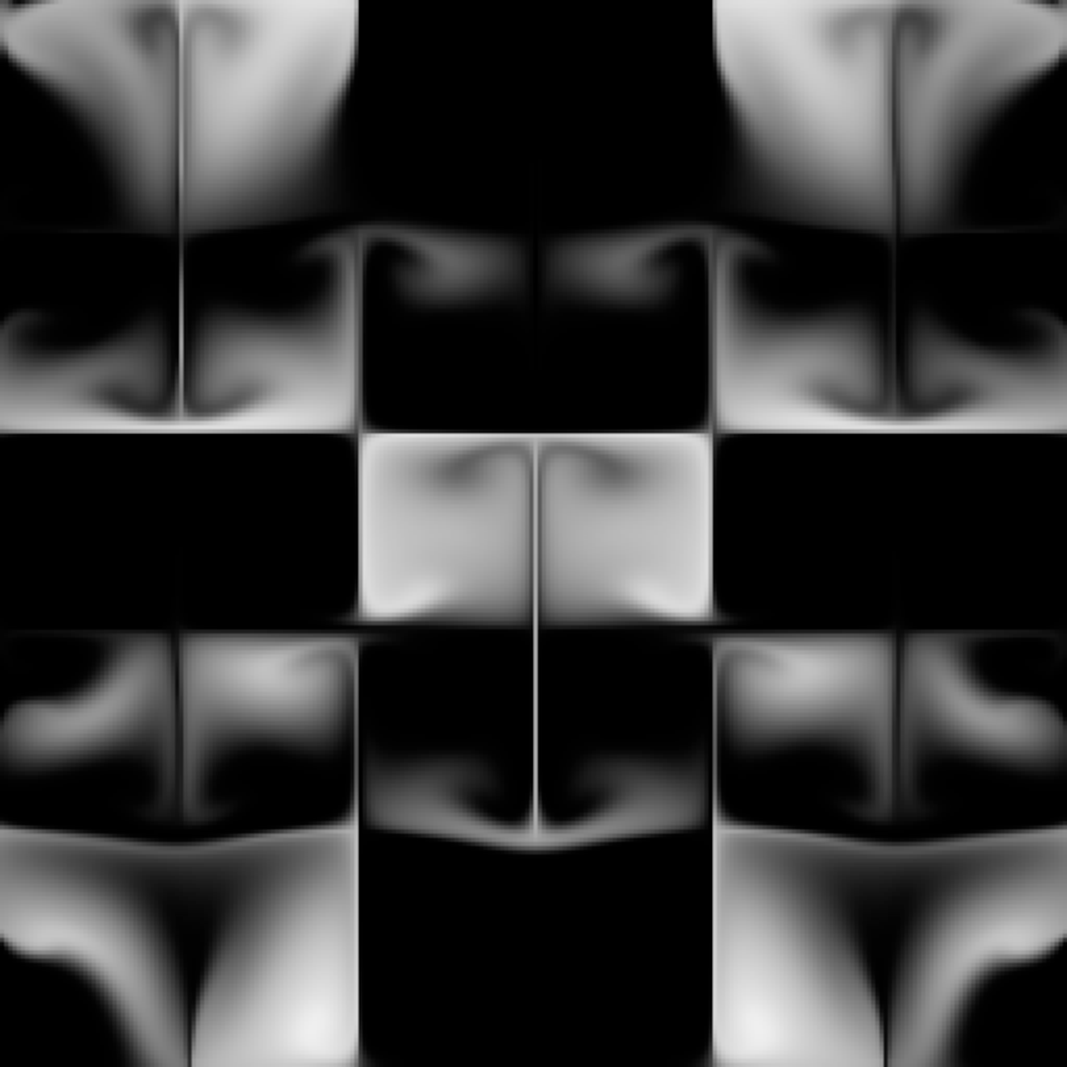
\includegraphics[width=0.3\textwidth]{images/sec-6/fluid/fluid-50}
        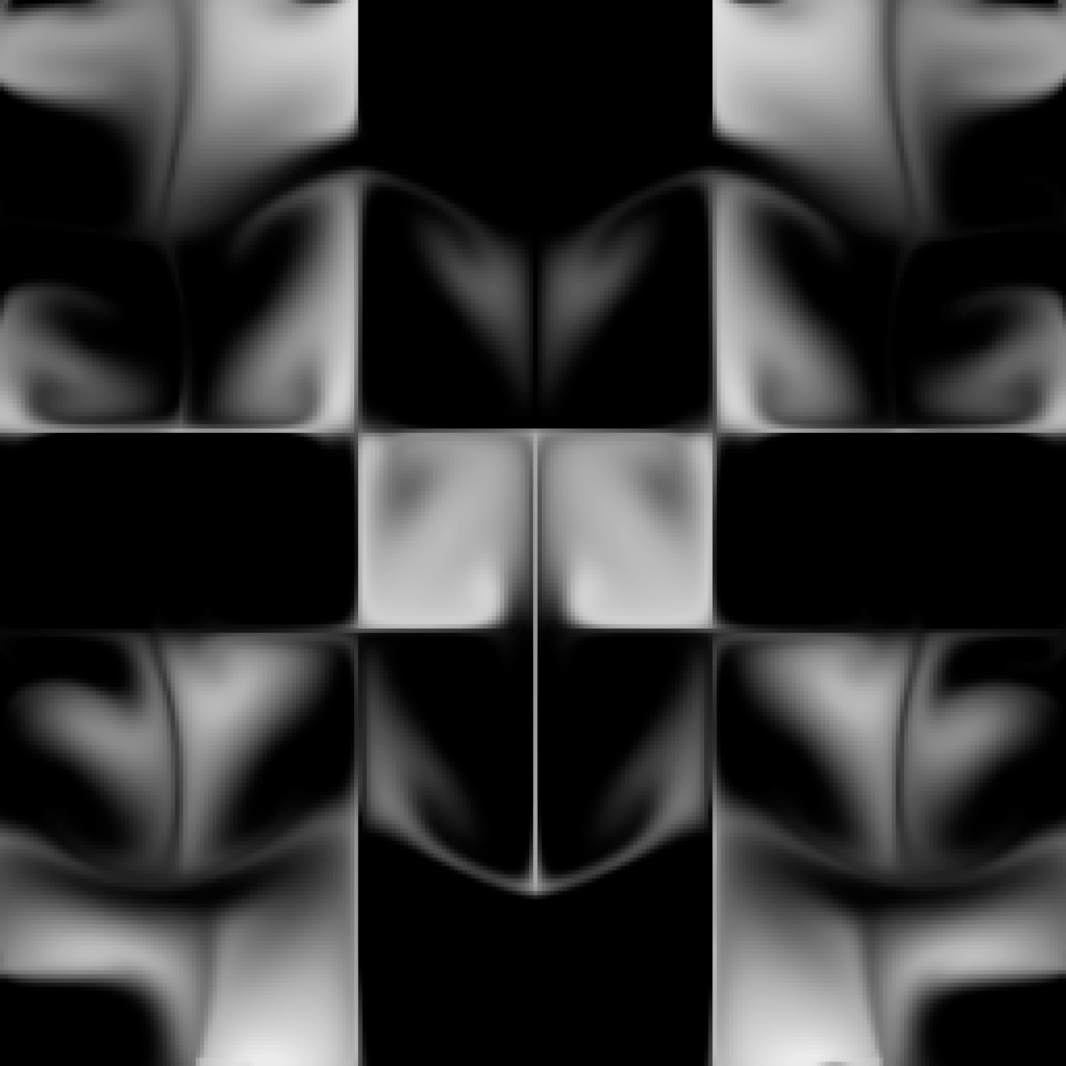
\includegraphics[width=0.3\textwidth]{images/sec-6/fluid/fluid-75}
    \end{center}
    \caption[Example of the fluid flow simulation]{An example showing the
        progression of the fluid flow simulation for a set of initial conditions
        after 10 (left), 50 (centre) and 75 (right) steps.}
    \label{fig:fluid_steps}
\end{figure}

The core of the algorithm is a finite time step simulation on a grid,
implemented as a matrix relaxation involving the discrete Laplace operator
($\nabla^2$). This step, known as the linear solver, is used to diffuse the
density and velocity fields throughout the grid, as well as apply a projection
operator to the velocity field to ensure it conserves mass. The linear solver is
implemented in terms of a stencil convolution, repeatedly computing the
following for each grid element to allow the solution to converge:
\[
u_{i,j}^{''} = \left( u_{i,j} + a \cdot \left( u'_{i-1,j}+u'_{i+1,j}+u'_{i,j-1}+u'_{i,j+1} \right) \right) / c
\]
Here, $u$ is the grid in the previous time step, $u'$ the grid in the current
time step and previous relaxation iteration, and $u''$ the current time step and
iteration. The values $a$ and $c$ are constants chosen by the simulation
parameters.

\begin{figure}[htbp]
    \begin{center}
        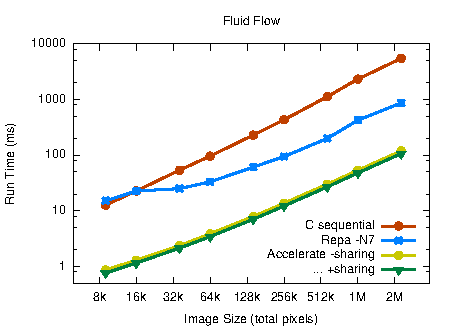
\includegraphics[width=0.8\textwidth]{images/sec-6/fluid/fluid}
    \end{center}
    \caption[Fluid flow simulation kernel benchmarks]{Kernel runtimes for the
        fluid flow simulation, in Accelerate with and without optimisations,
        compared to sequential and parallel CPU implementations. Running the
        Repa program with seven threads on the eight cores was found to be
        faster. Note the log-log scale.}
    \label{fig:fluid}
\end{figure}

Figure~\ref{fig:fluid} compares Accelerate to a parallel implementation written
in Repa and running on the host CPU \cite{Lippmeier:2012vv}. The program is
extremely memory intensive, performing approximately 160 convolutions of the
grid per time step. Given the nature of the computation, we find that the raw
bandwidth available on the CUDA device, which is much greater than that
available to CPU, results in correspondingly shorter run times. Since the
program consists of a sequence of stencil operations, fusion does not apply to
this program. Sharing recovery has a surprisingly minimal impact because the
implementation of stencils always shares some parts of the computation: namely
access to the grid elements $u_{xy}$, precisely because these operations are so
expensive.


\section{Canny edge detection}

The edge detection example applies the Canny algorithm to square images of
various sizes. The overall algorithm consists of seven distinct phases, the
first six of which are naturally data parallel and are performed on the GPU. The
last phase uses a recursive algorithm to ``connect'' the pixels that make up the
output lines. In our implementation this phase is performed on the CPU, which
requires the image data to be transferred from the GPU back to the CPU for
processing. In the figure, this final phase accounts for the non-linear slowdown
visible with smaller image sizes. We also show the run time for just the first
six data parallel phases, which exhibit linear speedup.

Neglecting the final phase, we note that the data parallel phase is still
slightly slower than in OpenCV. This is because the stencil kernels in
Accelerate currently make a test for every array access to see if the element is
in bounds, or if it lies outside the array and needs to be handled specially,
even though the vast majority of points in the array are far from the boundary.
For simple convolutions such as those used by Canny, this adds significant
overhead~\cite{BenLippmeier:2012cd}. To correct this infelicity we intend to
separate computation of the border region which requires boundary checks, from
the main internal region which does not, but leave this to future work.


\section{Radix sort}

The radix sort benchmark implements a simple parallel radix sort algorithm as
described by \citet{Blelloch:1990vl} to sort an array of signed 32-bit integers.
We compare our implementation of Blelloch's algorithm to one written in
Nikola~\cite{Mainland:2010vj}, which is also an embedded language in Haskell for
CUDA programming.\footnote{To be more specific, we estimate based on the results
presented in the paper~\cite{Mainland:2010vj} as Nikola no longer compiles with
recent versions of GHC, and the development version to replace it is not yet
complete. Nevertheless, results are informative as the same GPU, a Tesla T10, is
used in both cases.}
%
For this benchmark the Accelerate code is faster than Nikola, because Nikola is
limited to single kernel programs so must transfer every intermediate result
back to the host. Additionally, we are faster than a sequential radix sort
implementation using \texttt{Data.Vector} for as few as $\sim256$ elements,
whereas Nikola requires a dataset of about 32kB before the additional
parallelism of the GPU outperforms the sequential version.

Note that the absolute performance of this simple algorithm, which requires $b$
iterations to sort an array of elements $b$-bits wide, is quite low.
Implementations of radix sort optimised for the CUDA architecture, such as
Thrust~\cite{Satish:2009kx}, make efficient use of memory bandwidth and on-chip
shared memory and are approximately $10\times$ faster than Blelloch's algorithm
in Accelerate. To address this we propose to implement a foreign function
interface for Accelerate to take advantage of existing high-performance
libraries. We leave this for future work.


\section{Sparse-matrix vector multiplication}

\begin{table}
\centering
\begin{tabular}{lrrrr}

\textbf{Name}   & \parbox[b]{12ex}{\centering Non-zeros\\(nnz/row)}
                & \multicolumn{1}{c}{\rotatebox{90}{CUSP}}
                & \multicolumn{1}{c}{\rotatebox{90}{Accelerate}}
                & \multicolumn{1}{c}{\begin{sideways}\parbox{9ex}
                        {\centering Accelerate\\no fusion}\end{sideways}}
                \\ \hline

Dense                   & 4M (2K)       & 14.48 & 14.62 & 3.41  \\
Protein                 & 4.3M (119)    & 13.55 & 13.65 & 0.26  \\
FEM/Spheres             & 6M (72)       & 12.63 &  9.03 & 4.70  \\
FEM/Cantilever          & 4M (65)       & 11.98 &  7.96 & 4.41  \\
Wind Tunnel             & 11.6M (53)    & 11.98 &  7.33 & 4.62  \\
FEM/Harbour             & 2.37M (50)    &  9.42 &  6.14 & 0.13  \\
QCD                     & 1.9M (39)     &  7.79 &  4.66 & 0.13  \\
FEM/Ship                & 3.98 (28)     & 12.28 &  6.60 & 4.47  \\
Economics               & 1.27M (6)     &  4.59 &  0.90 & 1.06  \\
Epidemiology            & 1.27M (4)     &  6.42 &  0.59 & 0.91  \\
FEM/Accelerator         & 2.62M (22)    &  5.41 &  3.08 & 2.92  \\
Circuit                 & 959k (6)      &  3.56 &  0.82 & 1.08  \\
Webbase                 & 3.1M (3)      &  2.11 &  0.47 & 0.74  \\
LP                      & 11.3M (2825)  &  5.22 &  5.04 & 2.41  \\

\end{tabular}
\caption{Overview of sparse matrices tested and results of the benchmark.
Measurements are in GFLOPS/s (higher is better).}
\label{tab:smvm-summary}
\end{table}


This benchmark considers the multiplication of sparse matrices in compressed row
format (CSR)~\cite{Chatterjee:1990vj} with a dense vector. This matrix format
consists of an array of the non-zero elements paired with their column index,
together with a segment descriptor recording the number of non-zeros in each
row.

Table~\ref{tab:smvm-summary} compares Accelerate to the CUSP
library~\cite{Bell:2009}; a special purpose library for sparse matrix
operations. Using a 14 matrix corpus derived from a variety of application
domains~\cite{Williams:2009cy}, we compare against the CUSP implementation for
compressed row format matrices.

Compared to our previous work~\cite{Chakravarty:2011fr} the fusion
transformation compresses the program into a single segmented reduction. As
predicted, the corresponding reduction in memory bandwidth means that Accelerate
is on par with the CUSP library for several of the test matrices. In a balanced
machine SMVM should be limited by memory throughput, and a dense matrix in
sparse format should provide an upper bound on performance because loops are
long running and accesses to the source vector are contiguous and have high
re-use. We see that Accelerate with array fusion not only achieves this expected
performance limit, but is also slightly faster than the CUSP implementation.

However, matrices such as FEM/Spheres, with few non-zeros per row ($\lesssim 2
\times \text{warp size} = 64$) exhibit a drop in performance relative to CUSP.
This may be related to the way the skeleton code ensures that the vector read of
each row is coalesced and aligned to the warp boundary to maximise global memory
throughput, but is then not able to amortize this extra startup cost over the
row length. Matrices such as Epidemiology, with large vectors and few non-zeros
per row, exhibit low flop:byte ratio and are poorly suited to the CSR format,
with all implementations performing well below peak. The regression relative to
our previous result will be investigated. Nevertheless, this highlights the
nature of sparse computations and the reason the CUSP library supports several
algorithms and matrix formats.

